\newpage

\subsection{Building of TSEngine}
\label{sec:build}
The core of every modern C++ project is CMake % TODO:
% TODO: dll version

\subsection{Build Structure}
\label{sec:build_struct}
\begin{figure}
  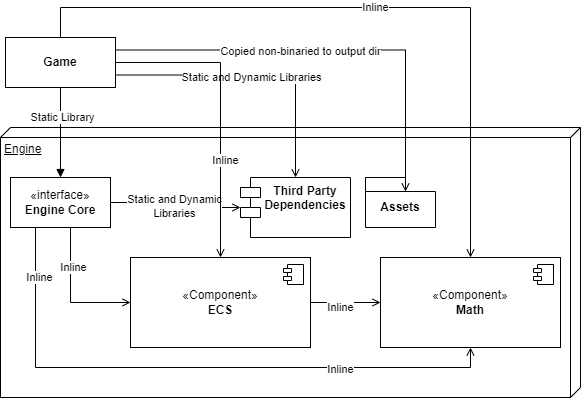
\includegraphics[width=\linewidth]{figures/build.png}
  \caption{Build Structure}
\end{figure}

\subsection{Instruction How To Run the Project}

\newpage
\subsubsection{Third Party Dependencies}
\label{lst:3rdparty}
We prioritize building from source code over using precompiled binaries % TODO: proses conses
One of the modern way of handling compiling from source code is to use git submodules. The core of this method is \texttt{.gitsubmodules} file containing all used external dependencies.
\begin{lstlisting}[caption=.gitsubmodules]
[submodule "external/vulkan"]
	path = external/vulkan
	url = https://github.com/KhronosGroup/Vulkan-Headers.git
[submodule "external/glslang"]
	path = external/glslang
	url = https://github.com/KhronosGroup/glslang
[submodule "external/googletest"]
	path = external/googletest
	url = https://github.com/google/googletest
[submodule "external/openxr"]
	path = external/openxr
	url = https://github.com/KhronosGroup/OpenXR-SDK.git
[submodule "external/tinyobjloader"]
	path = external/tinyobjloader
	url = https://github.com/tinyobjloader/tinyobjloader.git
\end{lstlisting}

\newpage
\subsubsection{Cyberith SDK}
There is one external dependency that git submodules doesn't cover, that dependency is Cybertith SDK, responsible for communication with Cyberith Virtualizer ELITE 2 treadmill.
This is the only 3rd party library that is included to the project as a binary and is optional to use.
More theory about this device and its SDK is available at:
\begin{itemize}
    \item \hyperref[]{Virtualizer} % TODO:
    \item \hyperref[sec:movement_system]{Movement System}
\end{itemize}

\newpage
\subsubsection{Precompiled header}

\newpage
\subsubsection{OS specific}
\label{sec:build_os}

\newpage
\subsubsection{CMake}
\begin{itemize}
    \item ./CMakeLists.txt
    \item ./external/CMakeLists.txt
    \item ./engine/CMakeLists.txt
        \begin{itemize}
            \item ./engine/tests/CMakeLists.txt
        \end{itemize}
    \item ./game/CMakeLists.txt
\end{itemize}

\newpage

\label{sec:abi}
\subsubsection{Common ABI}

\subsubsection{Preprocess definitions}

\subsubsection{Included directories}

\subsubsection{Unit Tests}
\label{sec:build_unit_tests}

\subsection{Source Control Version}
\subsubsection{GitHub Continuous intergration}
\subsubsection{.gitignore}